%\chapter{Introduction}
\label{chap_intro}

\textit{Disclaimer: This report is widely inspired by the review of Allahyari et al., A Brief Survey of Text Mining: Classification, Clustering and Extraction Techniques} \citep{Allahyari2017}.
\newline
\newline
In a very recent paper \citep{Tshitoyan2019}, researchers at Lawrence Berkeley National Laboratory have developed an artificial intelligence (AI) that paves the way to predict discoveries in science.
%\To spot what scientists had missed, all the AI had to do was read millions of previously published scientific papers. 
The scientists gathered 3.3 million articles on materials science from 1,000 different journals published between 1922 and 2018, and trained the renowned Word2vec algorithm in order to build statistical connections between words that are in the same context (\cf words embedding). 
%The renowned algorithm Word2vec was trained with abstracts published up to the year 2008, Word2vec was able to predict materials that appear in later from 2008 to 2018.
%\It took 500,000 distinct words from those abstracts and built mathematical connections between them. And that gave it very intriguing powers of prediction.
%\Based on the literature it analyzed, the AI was able to determine which material has the best thermoelectric properties. But it did something even more extraordinary. When fed abstracts published up to the year 2008, Word2vec was able to predict materials that appear in later studies.
\newline
On the one hand, the program was able to classify well known thermoelectric materials explicitly mentioned in the scientific abstracts alongside the word \doq thermoelectric\deq~or associated words like ‘ZT’, ‘zT’, ‘seebeck’, ‘thermoelectric’, ‘thermoelectrics’, ‘thermoelectrical’, ‘thermoelectricity’, ‘thermoelectrically’ or ‘thermopower’. However by mathematical projection of all the materials, it is also indicating a relationship that is not explicitly written in the text \fig~\ref{MaterialPrediction01}. Particularly \fig~\ref{MaterialPrediction01}-c demonstrates how words that are chemical formula, \ie totally new character strings, are associated through concept words expressing applications (electronic, optoelectronic, photovoltaic), physical parameters (bandgap, heusler compound) or others known thermoelectric material (PbTe, Cu\textsubscript{2}Te, Cu\textsubscript{5}Te\textsubscript{3}). 
\newline
On the other hand, articles from 2000 to 2018 were removed and 18 new predictive models were trained in order to predict discoveries the following years and evaluate prediction abilities (\figs~\ref{MaterialPrediction02} and \ref{MaterialPrediction03}).
Each of these models ranked materials according to their similarity to the word “thermoelectric” (or “ferroelectric”, “photovoltaic”, “topological insulator”), and took the top 50 that were not studied as thermoelectrics as of that year. It turns out, many of these materials were subsequently reported as thermoelectrics in future years.
\newline
%As many of you might have guessed, the brightest spots in the figure above are well known thermoelectric materials explicitly mentioned in the scientific abstracts alongside the word “thermoelectric”. However, some other bright spots have never been studied as thermoelectrics, so the algorithm is indicating a relationship that is not explicitly written in the text.
%\The amount of text that is generated every day is increasing dramatically. This tremendous volume of mostly unstructured text cannot be simply processed and perceived by computers.
%\The main source of machine-interpretable data for the materials research community has come from structured property databases. Beyond property values, publications contain valuable knowledge regarding the connections and relationships between data items as interpreted by the authors. To improve the identification and use of this knowledge, several studies have focused on the retrieval of information from scientific literature using supervised natural language processing, which requires large hand-labelled datasets for training.

%%%%%%%%%%%%%%%%%%%%%%%%%%%% FIGURE %%%%%%%%%%%%%%%%%%%%%%%%%%%%%%%%%
\begin{figure}[]
	\centering
	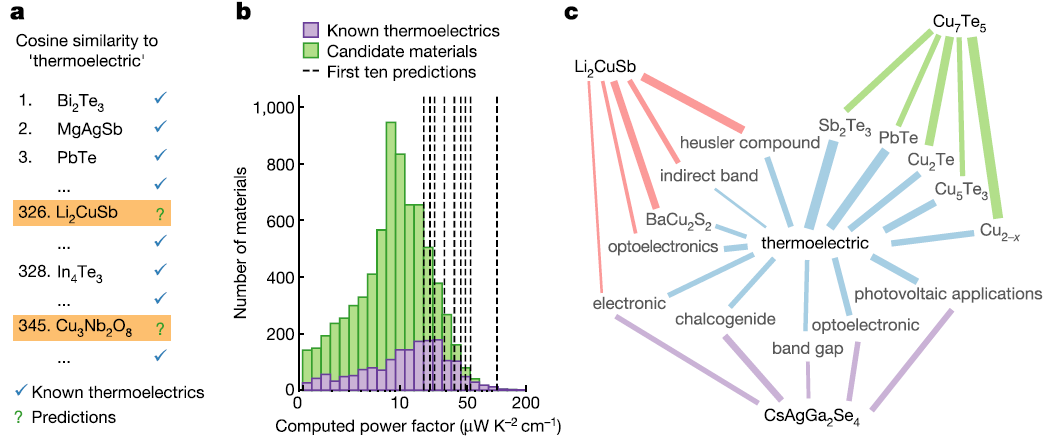
\includegraphics[width=1.0\textwidth]{imgs/Tshitoyan2019_Material_Predictions_01}
	\caption{Prediction of new thermoelectric materials based on 3.3 million scientific articles from 1,000 different journals published between 1922 and 2018 \citep{Tshitoyan2019}. 
		\newline
		\textbf{a.} Ranking table of thermoelectric materials. Materials with a check symbol are found in the context with thermoelectric terms (\ie ‘ZT’, ‘zT’, ‘seebeck’, ‘thermoelectric’, ‘thermoelectrics’, ‘thermoelectrical’, ‘thermoelectricity’, ‘thermoelectrically’ or ‘thermopower’). However materials with a interrogation point are not explicitly studied as thermoelectric but are \doq mathematically\deq{} close and potential predictions that can be tested in the future.
		\newline
		\textbf{b.} Distributions of the power factors (computed with specific chemistry calculations) for 1,820 known thermoelectrics in the literature (purple) and 7,663 candidate materials not yet studied as thermoelectric (green). Dashed lines show the 10 first predictions of table \textbf{a}: Li\textsubscript{2}CuSb \ldots
		\newline
		\textbf{c.} Graph showing how the context words of materials predicted to be thermoelectrics connect to the word thermoelectric. The materials are the first (Li\textsubscript{2}CuSb), third (CsAgGa\textsubscript{2}Se\textsubscript{4}) and fourth (Cu\textsubscript{7}Te\textsubscript{5}) predictions of table \textbf{a}. Examination of the context words demonstrates that the algorithm is making associations on the basis of crystal structure, co-mentions with other materials for the same application, between different applications and key phrases that describe the material’s known properties.
	}
	\label{MaterialPrediction01}
\end{figure}
%%%%%%%%%%%%%%%%%%%%%%%%%%%% FIGURE %%%%%%%%%%%%%%%%%%%%%%%%%%%%%%%%%
\begin{figure}[]
	\centering
	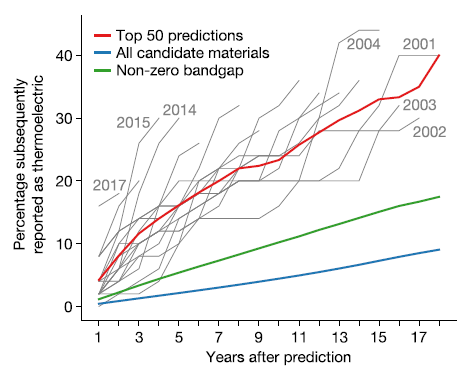
\includegraphics[width=0.6\textwidth]{imgs/Tshitoyan2019_Material_Predictions_02}
	\caption{Predictions of thermoelectric materials based on previously published papers  \citep{Tshitoyan2019}.
		\newline
		For example, predictions for 2001 are performed using abstracts from 2000 and earlier, and the grey lines plot the cumulative percentage of predicted materials subsequently reported as thermoelectrics in the years following their predictions.
		The results are averaged (red curve) and are 8 times more likely to have been studied as thermoelectrics within the next five years as compared to a randomly chosen unstudied material from our corpus at that time (blue curve) or three times more likely than a random material with a non-zero band gap (green curve).
	}
	\label{MaterialPrediction02}
\end{figure}
%%%%%%%%%%%%%%%%%%%%%%%%%%%% FIGURE %%%%%%%%%%%%%%%%%%%%%%%%%%%%%%%%%
\begin{figure}[]
	\centering
	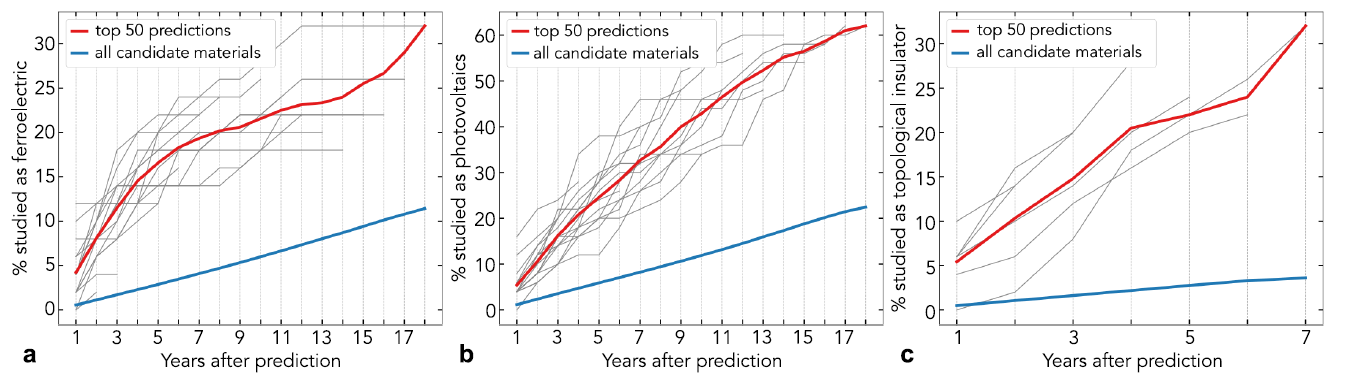
\includegraphics[width=1.0\textwidth]{imgs/Tshitoyan2019_Material_Predictions_03}
	\caption{Same prediction methods as \fig~\ref{MaterialPrediction02}, but with words related to ferroelectric (graph \textbf{a}), photovoltaic (graph \textbf{b}) and topological insulator  (graph \textbf{c}). 
	Supplementary material of \citep{Tshitoyan2019}.}
	\label{MaterialPrediction03}
\end{figure}


This work is perfect example of the target of the current work, \ie study future research and markets on a specific field that is here microfluidics. 

%%%%%%%%%%%%%%%%%%%%%%%%%%%% SECTION %%%%%%%%%%%%%%%%%%%%%%%%%%%%%%%%%
\section{Text mining}
%\section{Knowledge discovery vs. data mining}
Text Mining or knowledge discovery from text refers to the process of extracting high quality of information from structured database (i.e. RDBMS), semi-structured (\ie XML and JSON files), or unstructured text resources (\ie .pdf documents).
It widely covers a large set of related topics and algorithms for analyzing text, spanning various communities, including information retrieval, natural language processing, data mining, machine learning many application domains web and biomedical sciences.
\citeauthor{Allahyari2017} describe the notions of knowledge discovery, data mining, information retrieval, information extraction, text summarization or natural language processing in \citep{Allahyari2017}.

\subsection{Existing approaches}
\subsubsection{Unsupervised learning methods}
Unsupervised learning methods try to find hidden structure out of unlabeled data. Clustering and topic modeling are the two commonly used unsupervised learning algorithms used in the context of text data. 
\newline
Clustering is the task of segmenting a collection of documents into partitions where documents in the same group (cluster) are more similar to each other than those in other clusters. 
\newline
In topic modeling a probabilistic model is used to determine a soft clustering, in which every document has a probability distribution over all the clusters as opposed to hard clustering of documents. 
In topic models each topic can be represented as a probability distributions over words and each documents is expressed as probability distribution over topics. 
Thus, a topic is akin to a cluster and the membership of a document to a topic is probabilistic

\subsubsection{Supervised learning methods}
As aforementioned in the beginning of the introduction, supervised learning methods are machine learning techniques pertaining to infer a function or learn a classifier from the training data in order to perform predictions on unseen data. 
There is a broad range of supervised methods such as nearest neighbor classifiers, decision trees, rule-based classifiers and probabilistic classifiers.

\subsection{Some current applications}
Text processing 
\subsubsection{Natural Language Processing (NLP)}
\subsubsection{Text summarization}
\subsubsection{Text streams and social media mining}
\subsubsection{Opinion mining and sentiment analysis}

%%%%%%%%%%%%%%%%%%%%%%%%%%%% SECTION %%%%%%%%%%%%%%%%%%%%%%%%%%%%%%%%%
\section{Current work objective, database and approach}

\subsection{Objective}
The work targets to study scientific papers specialized in microfluidics and extract hot topics. 

On the one hand, amount of accessible texts has been increasing rapidly, and potentially contain a great wealth of knowledge.
On the other hand, analyzing huge amounts of textual data requires a tremendous amount of work in reading all of the text and organizing the content. Thus, the increase in accessible textual data has caused an in- formation flood in spite of hope of becoming knowledgeable about various topics.



\subsection{Text database}
First samples are from a conference proceedings specialized in microfluidics: MicroTAS or \textmu TAS (\appendice~\ref{Appendice_MicroTASpaper}, \url{http://microtas2019.org/}).
As undermentioned in following \chap, the text pre-processing is complex because of the text encoding of the .pdf files first and the heterogeneous paragraph sectioning by the authors. 

The second step is to analyze more microfluidics papers for scientific journals (\ie  \href{https://www.rsc.org/journals-books-databases/about-journals/lab-on-a-chip/}{RSC Lab-on-a-Chip}, \href{https://link.springer.com/journal/10404}{Springer Microfluidics and Nanofluidics} \ldots), and microfludics applications journals (\ie\textcolor{red}{à remplir} \ldots)
\newline

In both cases,  the access to the full text is quite expensive. However, in the case of journals, title, keywords and abstract are accessible on the internet and potentially in semi-structured files such as XML.

\subsection{Selected approach}
Probabilistic Methods for Text Mining: 
There are various probabilistic techniques including unsupervised topic models such as probabilistic Latent semantic analysis (pLSA) and Latent Dirichlet Allocation (LDA), and supervised learning methods such as conditional random fields that can be used regularly in the context of text mining.
